\section*{Methodology}

\begin{figure*}[ht]
\centering
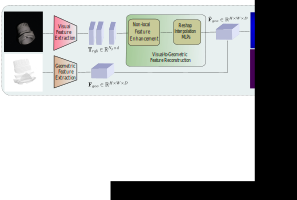
\includegraphics[width=\linewidth]{figs/overview}
\caption{Overview of the proposed unsupervised anomaly detection framework. The method extracts 2D visual features from RGB images and 3D geometric features from point clouds. A Visual-to-Geometric Feature Reconstruction network predicts geometric features from visual inputs, and significant discrepancies indicate anomalies.}
\label{fig:view}
\end{figure*}

Let $\mathbf{I} \in \mathbb{R}^{H \times W \times 3}$ represent an RGB image, where $H$ and $W$ denote the height and width of the image, and the 3 channels correspond to the color information. Let $\mathbf{D} \in \mathbb{R}^{H \times W}$ represent the corresponding depth image, which is pixel-registered with $\mathbf{I}$. This means that each pixel $(u, v)$ in $\mathbf{D}$ corresponds to a pixel in $\mathbf{I}$, providing a depth value $d_{u,v}$ for each valid pixel. From the depth image $\mathbf{D}$, we generate a 3D point cloud $\mathbf{P} = \{(x_i, y_i, z_i)\}_{i=1}^{M}$, where $M$ is the number of valid depth points and each point $(x_i, y_i, z_i)$ represents the 3D coordinates derived from the depth information.

As shown in Figure \ref{fig:view} the objective of the proposed method is to detect anomalies by predicting the 3D geometric features $\hat{\mathbf{F}}_{geo}$ from the 2D visual features $\mathbf{F}_{vis}$ and comparing them with the actual geometric features $\mathbf{F}_{geo}$ extracted from the point cloud. First, the visual features $\mathbf{F}_{vis} \in \mathbb{R}^{H \times W \times d}$ are extracted from the RGB image $\mathbf{I}$ using a Vision Transformer (ViT), capturing the appearance of the object in 2D space. Then, the 3D geometric features $\mathbf{F}_{geo} \in \mathbb{R}^{H \times W \times d}$ are obtained from the depth image $\mathbf{D}$ using a pre-trained 3D model. The core of the method is the geometric feature reconstruction network, which predicts the geometric features $\hat{\mathbf{F}}_{geo}$ from the visual inputs $\mathbf{F}_{vis}$. During training, the network minimizes the difference between the predicted geometric features $\hat{\mathbf{F}}_{geo}$ and the actual geometric features $\mathbf{F}_{geo}$ by minimizing the loss $\mathcal{L}_{geo}$. This process allows the network to learn the normal correlations between 2D visual data and 3D geometric data. During inference, anomalies are detected by comparing the predicted geometric features $\hat{\mathbf{F}}_{geo}$ with the actual geometric features $\mathbf{F}_{geo}$. Significant deviations between these features, measured using the Euclidean distance or another discrepancy measure, indicate abnormal regions in the object.

\subsection*{3D Point Cloud Feature Extraction}

The 3D point cloud $\mathbf{P} = \{(x_i, y_i, z_i)\}_{i=1}^{M}$ is processed using a Masked Autoencoder (MAE) \cite{pang2022masked}. The point cloud is first divided into patches using Farthest Point Sampling (FPS) and K-Nearest Neighbors (KNN). FPS selects $n$ points as patch centers, and KNN selects the $k$ nearest neighbors for each center:

\begin{equation}
    \mathbf{C_T} = \text{FPS}(\mathbf{P}), \quad \mathbf{C_T} \in \mathbb{R}^{n \times 3}
\end{equation}
\begin{equation}
    \mathbf{P}_{patch} = \text{KNN}(\mathbf{P}, \mathbf{C_T}), \quad \mathbf{P}_{patch} \in \mathbb{R}^{n \times k \times 3}
\end{equation}

\noindent The masked point patches are processed through PointNet \cite{qi2017pointnet} and the autoencoder to produce geometric features $\mathbf{G}_{geom} \in \mathbb{R}^{M \times D}$. The geometric features $\mathbf{G}_{geom} \in \mathbb{R}^{M \times d}$ are produced for each point in the point cloud. Since the 3D point cloud is derived from the depth image $\mathbf{D}$, we know the pixel coordinates $(u_i, v_i)$ of each 3D point $(x_i, y_i, z_i)$, allowing us to map the geometric features back to their corresponding pixel locations in the 2D image. Using this projection, we place the geometric features into a sparse 2D feature map $\mathbf{G}_{map} \in \mathbb{R}^{H \times W \times d}$, where the pixel $(u_i, v_i)$ contains the feature vector for point $i$.

\begin{equation}
\mathbf{G}_{map}[u_i, v_i, :] = \mathbf{G}_{geom}[i, :]
\end{equation}

\noindent For pixels without corresponding 3D points, we apply interpolation method as in \cite{wang2023multimodal} to propagate geometric features from neighboring pixels:

\begin{equation}
    \mathbf{F}_{geo} = \text{Interpolate}(\mathbf{G}_{map}) \in \mathbb{R}^{H \times W \times D}
\end{equation}

\subsection*{Visual Feature Extraction}

The RGB image $\mathbf{I}$ is processed using a Vision Transformer (ViT) \cite{dosovitskiy2020image} to extract high-level visual features. The image $\mathbf{I}$ is divided into non-overlapping patches of size $p \times p$, and each patch is flattened into a vector. A linear projection is applied to embed the patches into a $d$-dimensional feature space:

\begin{equation}
    \mathbf{x}_p = \text{Flatten}(\mathbf{I}) \in \mathbb{R}^{(H \times W) / p^2 \times (p \times p \times 3)}
\end{equation}

\noindent The set of embedded patches is passed through the transformer encoder to obtain RGB feature tokens:

\begin{equation}
    \mathbf{T}_{rgb} = ViT(\mathbf{x}_p) \in \mathbb{R}^{N_p \times d}
\end{equation}

\noindent where $N_p = \frac{H \times W}{p^2}$ is the number of patches and $d$ is the dimension of the feature vectors. 

\subsection*{Visual-to-Geometric Feature Reconstruction}

\begin{figure*}[ht]
\centering
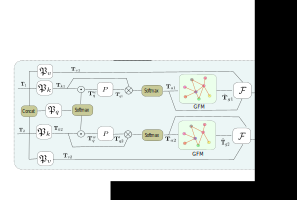
\includegraphics[width=0.8\linewidth]{figs/NL}
\caption{The proposed visual feature enhancement module $\mathcal{M}_{FE}$ used in geometric feature reconstruction. The module improves local feature representation through non-local attention and graph convolutional networks.}
\label{fig:NL}
\end{figure*}

While transformers excel at capturing global contextual information across the entire image, they often fall short when it comes to efficiently modeling local interactions. This becomes particularly problematic in anomaly detection, where distinguishing between normal and anomalous regions requires fine-grained analysis due to their often subtle differences. As a result, a combined approach that leverages both global context and local feature interactions is critical for achieving accurate detection. To address this challenge, we introduce a visual feature enhancement module $\mathcal{M}_{FE}$ that enhances the geometric feature reconstruction process by improving local feature representation (see Figure \ref{fig:NL}). Inspired by the works of \cite{te2020edge, wang2018non}, this module applies specialized operations to neighboring tokens, ensuring that localized details are preserved alongside the global context. The enhancement process begins with a non-local operation, which aggregates information from surrounding tokens to capture broader context and potential anomaly signals. Following this, a graph convolutional network (GCN) is employed to further explore the higher-order semantic relationships between neighboring tokens, allowing the model to detect subtle deviations that may indicate anomalies. The proposed enhancement method is particularly suitable for anomaly detection because anomalies typically manifest as small, localized changes in texture, structure, or geometry. The non-local operation ensures that the model can effectively consider both distant and nearby features, enabling it to detect anomalies that are not easily distinguishable based on local patterns alone. Meanwhile, the GCN enhances the model's ability to focus on higher-level semantic differences by refining local interactions, making it more sensitive to the fine-grained irregularities that characterize anomalies. Together, these operations create a robust system capable of detecting even subtle anomalies in complex industrial settings.

Specifically, given two neighboring tokens $\mathbf{T}_1$ and $\mathbf{T}_2$ from visual feature extraction, they are normalized. For instance, $\mathbf{T}_1$ is passed through two linear projection functions, $\mathfrak{P}_v$ and $\mathfrak{P}_k$, yielding dimension-reduced sequences $\mathbf{T}_v$ and $\mathbf{T}_k$ ($\mathbf{T}_v \in \mathbb{R}^{N_p \times \frac{d}{2}}$ and $\mathbf{T}_k \in \mathbb{R}^{N_p \times \frac{d}{2}}$):

\[
\mathbf{T}_v = \mathfrak{P}_v(\mathbf{T}_1), \quad \mathbf{T}_k = \mathfrak{P}_k(\mathbf{T}_1)
\]

\noindent Next, $\mathbf{T}_1$ and $\mathbf{T}_2$ are concatenated to form an integrated token $\mathbf{T}_q$. A linear projection $\mathfrak{P}_q$ reduces its dimension to $\frac{d}{2}$, and a softmax function produces a weight map $\mathbf{T}_q^w$. This map is element-wise multiplied with $\mathbf{T}_k$, followed by adaptive average pooling $P(\cdot)$ to reduce computational cost:

\[
\mathbf{T}_q' = F_1(\mathbf{T}_k, \mathbf{T}_q) = P\left(\mathbf{T}_k \odot \text{softmax}(\mathfrak{P}_q(\mathbf{T}_q))\right)
\]

\noindent A matrix product between $\mathbf{T}_k$ and $\mathbf{T}_q'$ explores their correlation, followed by a softmax operation to generate an attention map $\mathbf{T}_a$:

\[
\mathbf{T}_a = \text{softmax}\left(\mathbf{T}_q' \otimes \mathbf{T}_k^\top\right)
\]

\noindent Following \cite{te2020edge}, the attention map $\mathbf{T}_a$ and token $\mathbf{T}_v$ are passed to a graph fusion module (GFM). In GFM, $\mathbf{T}_v$ is projected onto the graph domain using $\mathbf{T}_a$:

\[
\mathbf{T}_g = \mathbf{T}_v \otimes \mathbf{T}_a^\top
\]

\noindent In this step, pixels with similar features are grouped into a vertex, and a single-layer GCN learns high-level semantic relations and non-local representations. The vertex features $\mathbf{T}_g$ undergo a spectral graph convolution, producing:

\[
\hat{\mathbf{T}}_g = \text{ReLU}\left((I - A)\mathbf{T}_g w_g\right)
\]

\noindent where $A$ is the adjacency matrix representing graph connectivity, and $w_g \in \mathbb{R}^{p \times p}$ is the GCN weight matrix. Finally, a skip connection combines the input token $\mathbf{T}_1$ with the enhanced representation:

\[
\mathbf{T}_{1}^{e} = \mathcal{F}_2(\hat{\mathbf{T}}_g, \mathbf{T}_a, \mathbf{T}_1) = \hat{\mathbf{T}}_g \otimes \mathbf{T}_a^\top + \mathbf{T}_1
\]

\noindent The same process is applied to other tokens. Since the number of patches $N_p$ is smaller than the spatial dimensions $H \times W$, each token in $\mathbf{T}^{e}$ corresponds to a $p \times p$ patch in the original image. To restore the resolution of the enhanced features, the tokens $\mathbf{F}_{e}$ are reshaped into a patch-based feature map:

\begin{equation}
    \mathbf{F}_{patches} = \text{Reshape}(\mathbf{T}^{e}) \in \mathbb{R}^{\frac{H}{p} \times \frac{W}{p} \times d}
\end{equation}

\noindent Next, the patch-based feature map is upsampled using bilinear interpolation to match the original image resolution:

\begin{equation}
    \mathbf{F}_{vis} = \text{BilinearUpsample}(\mathbf{F}_{patches}) \in \mathbb{R}^{H \times W \times d}
\end{equation}

\noindent This ensures spatial alignment of $\mathbf{F}_{vis}$ with the original image dimensions $H \times W$. Finally, a lightweight MLP maps the visual feature vector of size $d$ to the geometric feature of size $D$, producing the predicted geometric feature map $\hat{\mathbf{F}}_{geo} \in \mathbb{R}^{H \times W \times D}$. The L2 loss between the predicted and actual geometric features $\mathbf{F}_{geo}$ from the 3D point cloud is minimized during training:

\begin{equation}
\mathcal{L}_{geo} = \frac{1}{HWD} \sum_{i=1}^{H} \sum_{j=1}^{W} \sum_{k=1}^{D} \left( \mathbf{F}_{geo}(i, j, k) - \hat{\mathbf{F}}_{geo}(i, j, k) \right)^2
\end{equation}

\noindent The network progressively refines the visual features using convolutional layers, residual blocks, and attention mechanisms. By minimizing $\mathcal{L}_{geo}$, the network learns correlations between 2D appearance and 3D structure, making it highly effective for detecting anomalies in industrial settings. The combination of attention mechanisms and residual connections ensures the preservation and effective utilization of spatial and channel information during geometric feature prediction.

\subsection*{Anomaly Localization}

During inference, we use the trained prediction network to predict geometric features from the visual features of test samples. For each sample, we extract the 2D visual features $\mathbf{F}_{vis}$ from the RGB image using the pre-trained 2D model and the 3D geometric features $\mathbf{F}_{geo}$ from the point cloud using the pre-trained 3D model. The visual features $\mathbf{F}_{vis}$ are then passed through the geometric feature prediction network to predict the corresponding geometric features $\hat{\mathbf{F}}_{geo}$. We compute an anomaly map by measuring the difference between the predicted geometric features $\hat{\mathbf{F}}_{geo}$ and the actual geometric features $\mathbf{F}_{geo}$ at each spatial location using the L2 norm:

\begin{equation}
\mathbf{A}_{\text{anomaly}}(i, j) = \|\mathbf{F}_{geo}(i, j) - \hat{\mathbf{F}}_{geo}(i, j)\|_2
\end{equation}

\noindent This anomaly map $\mathbf{A}_{\text{anomaly}} \in \mathbb{R}^{H \times W}$ indicates the likelihood of anomalies at each spatial location. Regions with higher values represent areas where the predicted geometric features deviate significantly from the actual geometric features, suggesting the presence of anomalies. To obtain a global anomaly score for each sample, we calculate the maximum value in the anomaly map:

\begin{equation}
S_{\text{global}} = \max_{i,j} \mathbf{A}_{\text{anomaly}}(i, j)
\end{equation}

\noindent If the global anomaly score $S_{global}$ exceeds a predefined threshold, the sample is classified as anomalous. Additionally, the anomaly map provides spatial localization of anomalies by highlighting regions where the largest deviations occur, enabling a detailed inspection of the anomalous areas. This method effectively localizes anomalies by leveraging the learned mapping between 2D visual features and 3D geometric features, making it possible to detect deviations in both the appearance and structure of objects in industrial anomaly detection tasks.
